\rhead{\'ECOULEMENTS DIPHASIQUES}
\chapter{\label{sec:CMFD}Computational Multiphase Fluid Dynamics}
\lhead{CMFD}
\section{Turbulence implementation in TrioCFMD}
A CFD module, called CMFD (Computaional Multiphase Fluid Dynamics) is currently under development and will be able to handle single and multi-phase turbulent flows. TrioCMFD uses the PolyMAC numerical scheme \cite{Gerschenfeld_PolyMAC2018, Gerschenfeld_PolyMAC2022}. This scheme was initially developed for component scale codes. The resolution of the equations is done using semi-implicit ICE and SETS solvers. Turbulence is treated through two-equation models. There is an equation on the turbulent kinetic energy $k$ and one on the turbulent dissipation rate $\omega$ or time scale $\tau$. The equations for turbulent quantities are treated in the same way as the conservation equation for energy and solved in a Newton algorithm in the same matrix as the mass, velocity, pressure and temperature equations. \\

Turbulence acts on the momentum equation through a modified diffusivity as per the eddy-viscosity hypothesis. It acts on the energy equation through a SGDH transport term of which the user can tune the Prandtl number. \\

Work is still being done on the models presented in this section, and they are not fully validated. Datasets can be found in triocfd-code/Multiphase/CMFD/share/Validation/Rapports\_automatiques/ to launch calculations.
\newpage

\subsection{Definition of dimensionnal and dimensionless variables}

\begin{center}
\begin{tabular}{|r|l|}
	\hline Variable name & Expression \\ \hline \hline
	Distance from the face to the element & $y$ \\ \hline
	Normal unit vector of the face & $\overrightarrow{n}$ \\ \hline
	Velocity at the element center & $\overrightarrow{u}$\\ \hline
	Perpendicular velocity at the element center 
		& $\overrightarrow{u_{\perp}}=u_{\perp}\overrightarrow{n}$\\ \hline
	Parallel velocity at the element center 
		& $\overrightarrow{u_{\parallel}}=\overrightarrow{u} - (\overrightarrow{u}\cdot\overrightarrow{n})\overrightarrow{n}$\\ \hline
	Tangent unit vector 
		& $\overrightarrow{t} = \overrightarrow{u_{\parallel}}/u_{\parallel}$ \\ \hline
	Hydraulic diameter
		& $D_h$ \\ \hline
	Dynamic viscosity in the element
		& $\mu $ \\ \hline
	Volume mass in the element
		& $\rho$ \\ \hline
	Kinematic viscosity in the element 
		& $\nu = \mu/\rho$ \\ \hline
	Turbulent dynamic viscosity in the element
		& $\mu_{t} $ \\ \hline
	Turbulent kinematic viscosity in the element 
		& $\nu_t = \mu_t/\rho$ \\ \hline
	Dimensionless turbulent kinematic viscosity in the element 
		& $\nu_{t+} = \nu_t/\nu = \partial_{u_+}y_+ - 1$ \\ \hline	
	Shear stress at the face 
		& $\overrightarrow{\tau_f} = -\tau_f \overrightarrow{t}$ \\ \hline
	Friction velocity 
		& $u_\tau = \sqrt{\tau_f/\rho}$ \\ \hline
	Dimensionless distance from face to element
		& $y_+ = y u_tau / \nu$ \\ \hline
	Dimensionless velocity
		& $u_+ = u_{\parallel}/u_\tau$ \\ \hline
	Turbulent kinetic energy 
		& $k$ \\ \hline
	Dimensionless turbulent kinematic energy 
		& $k_+ = k/u_\tau^2$ \\ \hline
	Turbulent dissipation frequency
		& $\omega$ \\ \hline
	Dimensionless turbulent dissipation frequency
		& $\omega_+ = u_\tau^2/\nu$ \\ \hline
	Turbulent time scale
		& $\tau = 1/\omega$ \\ \hline
	Dimensionless turbulent time scale
		& $\tau_+ = 1/\omega_+$ \\ \hline 
	Temperature in the element 
		& $T$ \\ \hline
	Temperature in the fluid at the wall
		& $T_w$ \\ \hline
	External temperature, i.e. temperature of the wall
		& $T_{\text{ext}}$ \\ \hline
	Thermal conductivity
		& $k_T =$ \\ \hline
	Heat capacity at constant volume
		& $C_p$ \\ \hline
	Thermal diffusivity
		& $\lambda = k_T/(\rho C_p)$ \\ \hline
	Heat transfer coefficient
		& $h$	\\ \hline
	Heat flux
		& $q = h\cdot(T_\text{ext}-T)$ \\ \hline
	Characteristic temperature
		& $T_* = q/(\rho C_p u_\tau) $ \\ \hline
	Dimensionless temperature difference
		& $\theta_+ = (T_\text{ext}-T) /T_*$ \\ \hline
	Prandtl number
		& $Pr = \nu/\lambda$ \\ \hline
	Turbulent Prandtl number
		& $Pr_t = \nu_t/\lambda_t$ \\ \hline
	Von Karman constant
		& $\kappa = 0.41$ \\ \hline
	Liquid fraction 
		& $\alpha_l $ \\ \hline

\end{tabular}
\end{center}
\pagebreak

\subsection{Turbulence models implemented in TrioCMFD}

All of the constants used in the models are user-defined in the calculation dataset. This enables an easy transition from one turbulence model to another. The models that one can use to launch a calculation are the following.

\subsubsection{1988 Wilcox $k-\omega$}

This is one of the first models that uses $\omega$ and not $\epsilon$ to model the energy dissipation \cite{Wilcox1988}. Here, $\nu_t = \frac{k}{\omega}$. The turbulent equations are:

\begin{equation}
	\begin{split}
		\partial_t \rho_l k + \nabla \cdot ( \rho_l k \vec{u_l}) =  
		& { \underline{\underline{\tau_R}}::\underline{\underline{\nabla}}\vec{u_l} }
		{ - \beta_{k}\rho k \omega }
		{ + \nabla( \rho_l(\nu_l + \sigma_k \nu_t) \underline{\nabla} k) } 
		\\
		\partial_t  \rho_l \omega + \nabla \cdot (\alpha_l \rho_l \omega \vec{u_l}) =
		& { \alpha_{\omega}  \frac{\omega}{k}\underline{\underline{\tau_R}}::\underline{\underline{\nabla}}\vec{u_l} }
		{ - \beta_{\omega}\rho \omega^2 }
		{ +\nabla(  \rho_l(\nu_l + \sigma_{\omega} \nu_t) \underline{\nabla} \omega) }
	\end{split}
\end{equation}

The values of the constants are $\alpha_{\omega} = 0.55$, $\beta_{k} = 0.09$, $\beta_{\omega} = 0.075$, $\sigma_k = 0.5$ and $\sigma_{\omega} = 0.5$.

\subsubsection{Kok $k-\omega$}

This model \cite{Kok1999} was introduced after the Menter SST $k-\omega$ model \cite{Menter1993, Menter2003} showed the importance of cross-diffusion. The differences with the 1988 Wilcox model reside in the addition of a cross-diffusion term (${ \sigma_d\frac{  \rho_l}{\omega} } \text{max}\left\{{\underline{\nabla}k \cdot \underline{\nabla} \omega}, 0\right\}  $) and a modification of the value of some constants. The turbulent equations are:

\begin{equation}
	\begin{split} \label{eq_omega_Kok}
		\partial_t \rho_l k + \nabla \cdot ( \rho_l k \vec{u_l}) =  
		& { \underline{\underline{\tau_R}}::\underline{\underline{\nabla}}\vec{u_l} }
		{ - \beta_{k}\rho k \omega }
		{ + \nabla( \rho_l(\nu_l + \sigma_k \nu_t) \underline{\nabla} k) } 
		\\
		\partial_t  \rho_l \omega + \nabla \cdot (\alpha_l \rho_l \omega \vec{u_l}) =
		& { \alpha_{\omega}  \frac{\omega}{k}\underline{\underline{\tau_R}}::\underline{\underline{\nabla}}\vec{u_l} }
		{ - \beta_{\omega}\rho \omega^2 }
		{ +\nabla(  \rho_l(\nu_l + \sigma_{\omega} \nu_t) \underline{\nabla} \omega) }
		+ { \sigma_d\frac{  \rho_l}{\omega} } \text{max}\left\{{\underline{\nabla}k \cdot \underline{\nabla} \omega}, 0\right\}  
	\end{split}
\end{equation}

The values of the constants are	$\alpha_{\omega} = 0.5$, $\beta_{k} = 0.09$, $\beta_{\omega} = 0.075$, $\sigma_k = 2/3$, $\sigma_{\omega} = 0.5$ and $\sigma_d = 0.5$.

\subsubsection{Kok $k-\tau$}

This is a variation of the 1999 Kok $k-\omega$. In this model \cite{Ktau2000}, the time scale $\tau = \frac{1}{\omega}$ is introduced. We therefore have $\nu_t = k\tau$. There is an additional diffusion term that comes out of the calculation ( $- 8  \rho_l(\nu_l + \sigma_{\omega} \nu_t) ||\underline{\nabla}\sqrt{\tau}||^2$). The turbulent equations become:

\begin{equation} \label{eq_tau}
\begin{split}
		\partial_t \rho_l k + \nabla \cdot ( \rho_l k \vec{u_l}) 
		= &  { \underline{\underline{\tau_R}}::\underline{\underline{\nabla}}\vec{u_l} }
		{ - \frac{\beta_{k}\rho k}{\tau} }
		{ + \nabla(  \rho_l(\nu_l + \sigma_k \nu_t) \underline{\nabla} k)}
		\\
		\partial_t  \rho_l \tau + \nabla \cdot ( \rho_l \tau \vec{u_l})
		= & { - \alpha_{\omega}  \frac{\tau}{k}\underline{\underline{\tau_R}}::\underline{\underline{\nabla}}\vec{u_l} }
		{ + \beta_{\omega}\rho }
		{ +\nabla(  \rho_l(\nu_l + \sigma_{\omega} \nu_t) \underline{\nabla} \tau)} \\
		& { + \sigma_d \rho_l \tau \text{min}\left\{\underline{\nabla}k \cdot \underline{\nabla} \tau, 0\right\} }
		- 8  \rho_l(\nu_l + \sigma_{\omega} \nu_t) ||\underline{\nabla}\sqrt{\tau}||^2
\end{split}
\end{equation}

The $- 8  \rho_l(\nu_l + \sigma_{\omega} \nu_t) ||\underline{\nabla}\sqrt{\tau}||^2$ term presents important numerical difficulties close to the wall. In order to limit these issues, we have tried to implicit this term in 3 different ways. The comparison between these methods and the determination of the most robust solution is ongoing.\\

The constants are the same than in the 1999 Kok $k-\omega$ model: $\alpha_{\omega} = 0.5$, $\beta_{k} = 0.09$, $\beta_{\omega} = 0.075$, $\sigma_k = 2/3$, $\sigma_{\omega} = 0.5$, $\sigma_d = 0.5$.

\subsubsection{2006 Wilcox $k-\omega$}

The 2006 Wilcox $k_\omega$ model \cite{Wilcox2006} is the same as the Kok $k_\omega$ with different coefficients. It is an update of the 1988 Wilcox $k-\omega$ model. The turbulent equations are the same as in equation \ref{eq_omega_Kok}. A notable difference is the introduction of a blending function for $\beta_{\omega}$. \\

The values of the constants are: $\alpha_{\omega} = 0.52$, $\beta_{k} = 0.09$, $\beta_{\omega} = 0.0705\cdot f(\Omega_{ij},S_{ij})$, $\sigma_k = 0.6$, $\sigma_{\omega} = 0.5$ , $\sigma_d = 0.125$.

\subsection{Boundary conditions implemented in TrioCMFD}

The boundary conditions at the wall for elements small enough to be in the viscous regime are usually $\overrightarrow{u} = 0$, $T = T_{\text{wall}}$, $k=0$, $\tau = 0$, and something smart for $\omega$ ($\omega \rightarrow +\infty$ when $y\rightarrow0$).\\

When the first element is too large for the viscous regime to be valid, different boundary conditions must be implemented. 

\subsubsection{Velocity}

The viscous boundary condition on velocity is:
\begin{equation} \label{velocity_0}
	\overrightarrow{u} = 0
\end{equation}

The velocity function used in many codes when the first element is large is the log-law. We have:

\begin{equation}
	u_{+\text{Log}} = \frac{1}{\kappa}\text{ln}(y_+) + 5.1
\end{equation}

However, this is valid only for $30 \lesssim y_+ \lesssim 300$. In 1951, Reichardt \cite{Reichardt1951} proposed a formulation valid for smaller $y_+$:

\begin{equation}
	u_{+\text{Rei}} = \frac{1}{\kappa}\text{ln}(1+0.4y_+) + 7.8\left(1-\text{exp}(-y_+/11)-\frac{y_+}{11}\text{exp}(-y_+/3)\right)
\end{equation}

Here, we use a blending proposed by Knopp  \cite{Knopp2007} that is used in the Fun3D code \cite{Fun3D2015}:

\begin{equation}
	\phi = \text{tanh}\left[\left(\frac{y_+}{27}\right)^4\right]
\end{equation}
\begin{equation}\label{velocity_Knopp}
	u_+ = \phi u_{+\text{Log}} +(1-\phi) u_{+\text{Rei}}
\end{equation}

The boundary condition is enforced through the calculation of a shear stress that is calculated knowing $u_{\parallel}$ in the first element.\\

\begin{figure}[h]
	\centering
	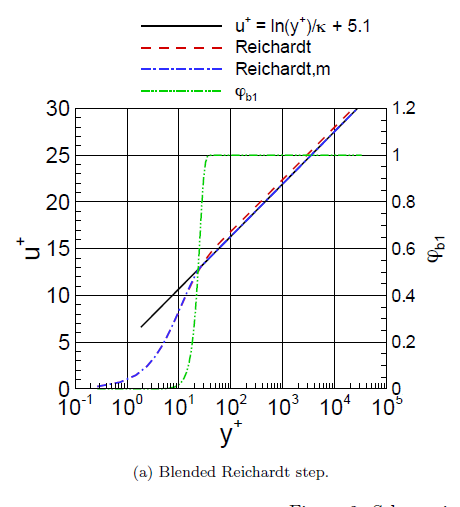
\includegraphics[width= 5cm]{Fun3D_v.png}
	\caption{RANS direct integration of the equations vs the Knopp proposal (figure from \cite{Knopp2007}).}
\end{figure}

For now, the boundary conditions that are implemented in TrioCMFD are equations \eqref{velocity_0} and \eqref{velocity_Knopp}.

\subsubsection{Turbulent kinetic energy}


Kalitzin et. al. \cite{Kalitzin2005} give a complete overview of the possible boundary conditions on the turbulent kinetic energy. Inside the viscous sublayer, the boundary condition on $k$ is:
\begin{equation}\label{eq_k_visc}
	k_{visc} = 0
\end{equation}

In the log-law region, the boundary condition is:
\begin{equation}\label{eq_k_log}
	k_{+,log} = 1/\sqrt{\beta_k}
\end{equation}

One of the often used proposals is:
\begin{equation}\label{eq_k_0}
	\partial_y k =0
\end{equation}

However, there is no universally accepted blending function. Another proposal is to use the relation $\nu_{t+} = \partial_{u_+}y_+ - 1$, but this has not been validated in a commercial code. This would yield:
\begin{equation}
	k_+ = \nu_{t+}\omega_+ = (\partial_{u_+}y_+ - 1) \omega_+
\end{equation}
\begin{equation}\label{eq_k_weak}
	\partial_y k_+ = (\partial_{u_+}y_+ - 1) \frac{u_\tau^2}{\nu} \partial_y \omega 
	- \frac{u_\tau}{\nu}\frac{\partial_{y_+}^2 u_+}{(\partial_{y_+}u_+)^2} \omega_+
\end{equation}

The formulations in equations $\eqref{eq_k_visc}$ and $\eqref{eq_k_0}$ are implemented in TrioCMFD. \\

Another simple boundary condition is a home-made transition from the viscous boundary condition to the zero-flux boundary condition by imposing a flux at the wall:
\begin{equation}\label{eq_k_blending}
	\Phi_{k, wall} = (\nu_l + \nu_t)/y \cdot (1-\tanh((y_+/20)^2))
\end{equation}

Finally, a boundary condition of equation \ref{eq_k_weak} is implemented with an imposed $k$ flux (see \cite{Mierka2007} for details on weak wall laws).

\subsubsection{Turbulent dissipation rate $\omega$}

The treatment of $\omega$ at the wall is one of the difficulties of $k-\omega$ models, as $\omega\rightarrow+\infty$ at the wall. \\

Wilcox recommends to input the values of $\omega$ in the first element by using the theoretical value of the viscous sub-layer: 
\begin{equation}
	\omega_\text{element} = \frac{6\nu}{\beta_\omega y^2}
\end{equation}

The boundary condition recommended by Menter in an SST $k-\omega$ \cite{Menter1993} is at the wall: 
\begin{equation}
	\omega_\text{wall} = 10 \frac{6\nu}{\beta_\omega y^2}
\end{equation}

Knopp proposed a blending function between the viscous and log-law regimes to obtain of $\omega$ \cite{Knopp2007}:

\begin{equation}
	\phi = \text{tanh}\left[\left(\frac{y_+}{10}\right)^2\right]
\end{equation}
\begin{equation}
	\omega_{vis} = \frac{6\nu}{\beta_\omega y^2}
\end{equation}
\begin{equation}
	\omega_{log} = \frac{u_\tau}{\sqrt{\beta_k}\kappa y}
\end{equation}
\begin{equation}
	\omega_{1} = \omega_{vis}+\omega_{log}
\end{equation}
\begin{equation}
	\omega_{2} =(\omega_{vis}^{1.2}+\omega_{log}^{1.2})^{1/1.2}
\end{equation}

\begin{equation}\label{eq_omega_Knopp}
	\omega = \phi \omega_{1} + (1-\phi) \omega_{2}
\end{equation}

They also recommend to enforce the theoretical value of $\omega$ in the first element. This is also what is done in \cite{Fun3D2015}. \\

\begin{figure}[h]
	\centering
	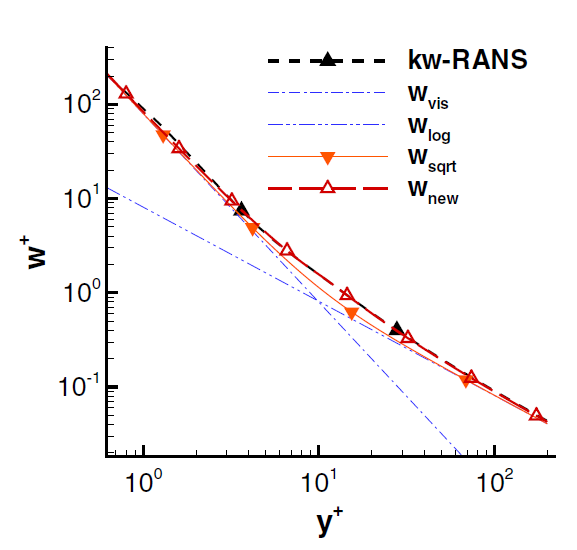
\includegraphics[width= 5cm]{Knopp_omega.png}
	\caption{RANS direct integration of the equations vs the Knopp proposal (image from \cite{Knopp2007}).}
\end{figure}

It is also possible to calculate the derivative of this theoretical value to obtain a flux to input in the first element:

\begin{equation}
	\partial_y\phi = \frac{u_\tau}{10\nu}\left(1-\text{tanh}\left[\left(\frac{y_+}{10}\right)^4\right]^2\right)
\end{equation}
\begin{equation}
	\partial_y\omega_{vis} = -\frac{12\nu}{\beta_\omega y^3}
\end{equation}\begin{equation}
	\partial_y\omega_{log} = - \frac{u_\tau}{\sqrt{\beta_k}\kappa y^2}
\end{equation}
\begin{equation}
	\partial_y\omega_{1} = \partial_y\omega_{vis}+\partial_y\omega_{log}
\end{equation}
\begin{equation}
	\partial_y\omega_{2} =(\omega_{vis}^{1.2}+\omega_{log}^{1.2})^{1/1.2}
\end{equation}
\begin{equation} \label{eq_omega_weak}
	\partial_y\omega = \partial_y\phi \omega_{1} + \phi \partial_y\omega_{1} -\partial_y\phi \omega_{2} + (1-\phi) \partial_y \omega_{2}
\end{equation}

For now, the only boundary condition that is implemented is \eqref{eq_omega_weak}, but work is ongoing on other possible boundary conditions.

\subsubsection{Turbulent time scale $\tau$}

The simplest boundary condition on $\tau$ is:
\begin{equation}\label{eq_tau_0}
	\tau_{wall}=0
\end{equation}

This is used in \cite{NEK50002020} for example. \\

Another possibility is to enforce a weak boundary condition by using $\tau = \frac{1}{\omega}$. This gives us:
\begin{equation}\label{eq_tau_weak}
	\partial_y\tau = -\frac{\partial_y\omega}{\omega^2}
\end{equation}

For now, the boundary conditions implemented on tau are \eqref{eq_tau_0} and \eqref{eq_tau_weak}. Work is ongoing on other possible boundary conditions.

\subsubsection{Temperature}

The heat transfer coefficient that we have implemented is the one proposed by Kader \cite{Kader1981}. It is compatible with adaptive wall functions. It is based on experiments and was later confirmed by DNS \cite{Mitrovic2004}. It is valid in an range where $6\cdot10^{-3}\inf Pr<6\cdot4^{4}$, for $Pr_t\approx0.85$.

\begin{equation}
	\Gamma = \frac{10^{-2}(Pr y_+)^4}{1+5Pr^3y_+}
\end{equation}
\begin{equation}
	\beta = (3.85Pr^{1/3}-1.3)^2+2.12ln(Pr)
\end{equation}
\begin{equation}
	\theta_+ = Pr y_+ \text{exp}(-\Gamma) +\left\{ 2.12ln\left[(1+y_+)\frac{2.5(2-2y/D_h)}{1+4(1-2y/D_h)^2}\right]+\beta\right\}\text{exp}(-1/\Gamma)
\end{equation}

\begin{figure}[h]
	\centering
	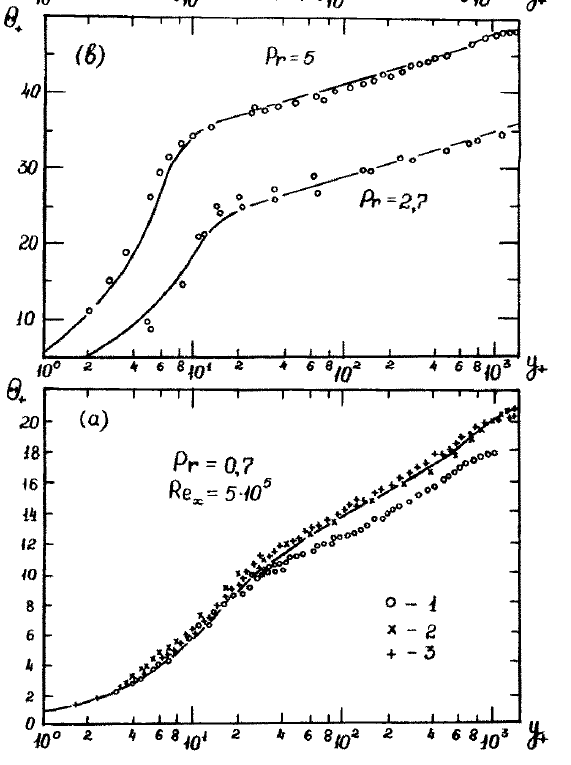
\includegraphics[width= 5cm]{Kader_T.png}
	\caption{Experimental results vs Kader forumala for different Prantl numbers (figure from \cite{Kader1981}).}
\end{figure}

\subsection{Description of the wall law algorithm implemented in TrioCMFD}

\subsubsection{Historic TrioCFD algorithm in VEF}

In VEF, the turbulent model used is $k-\epsilon$. The velocity is defined as a vector located at the center of the faces. Turbulent quantities (i.e. $k$ and $\epsilon$) as well. The information present in this subsection was determined by reading the source code.

For the velocity equation:
\begin{enumerate}
\item Calculate turbulent quantities at each face that is connected to a boundary element:
\begin{enumerate}
	\item Calculate $u_\parallel$ at the center of the face
	\item Calculate the friction viscosity $u_\tau$ using an iterative method that reconstructs the complete viscous sublayer, using $\frac{u_\parallel}{u_\tau} = u_+(\frac{y u_\tau}{\nu})$
	\item Calculate the shear stress $\tau_f = \rho u_\tau^2$
\end{enumerate}

\item Calculate the velocity diffusion terms:
\begin{enumerate}	
	\item Calculate the velocity diffusion for a $u=0$ boundary condition on the whole domain
	\item In the boundary elements, retract from the velocity diffusion the (viscosity * velocity gradient)  at the boundary face terms. Input the shear stress calculated with the wall law instead.
\end{enumerate}

\item Iterate one time step of the momentum equation

\item Update the turbulent quantity boundary conditions:
\begin{enumerate}
	\item Iterate one time step of the transport equation for $k$ and $\epsilon$.
	\item Use the equations on the turbulent quantities presented above to determine $\epsilon(y)$ and $k(y)$ at the faces connected to boundary elements.
	\item Input them in said faces at the end of each iteration (during the iterations, they are free to move as TrioCFD isn't designed to fix values inside elements or on faces as this would create a specific treatment for some internal faces and elements).
\end{enumerate}
\end{enumerate}

In VEF, the temperature is also located at the faces. To calculate the temperature diffusion, TrioCFD uses a separate equation to calculate the turbulence on temperature, recalculating $u_\tau$, $k$ and $\epsilon$ at the faces connected to a boundary element. Usually a Prandtl turbulence model is used to save calculation costs. When $k-\epsilon$ is used:
\begin{enumerate}
	\item Calculate $u_\tau$ in the faces connected to a boundary edge as for the velocity equation
	\item Calculate an equivalent distance to the edge using $u_tau$ to have the right heat flux while still using $T_{\text{wall}}$ at the edge in the diffusion operator.
	\item Iterate one time step of the conservation equation on the temperature.
	\item Iterate the equations for $k$ and $\epsilon$ as above.
\end{enumerate} 

\subsubsection{Fun3D algorithm}

See \cite{Fun3D2015}.

\begin{enumerate}
	\item Calculate $u_\parallel$
	\item Calculate the friction viscosity $u_\tau$ using Newton's method, using $\frac{u_\parallel}{u_\tau} = u_+(\frac{y u_\tau}{\nu})$
	\item Calculate the shear stress $\tau_f = \rho u_\tau^2$
	\item Obtain the momentum flux from the wall $-\tau_f \overrightarrow{t}$
	\item No heat transfer
	\item Turbulent quantities BL: it seems $\omega_{\text{element}} = \omega_{theorical}$ from equation \eqref{eq_omega_Knopp}, $k{\text{wall}} = 0$ are used (unclear in the paper)
\end{enumerate}

\subsubsection{TrioCMFD algorithm}

\begin{enumerate}
	\item Calculate $u_\parallel$
	\item Calculate the friction viscosity $u_\tau$ using dichotomic algorithm, using $\frac{u_\parallel}{u_\tau} = u_+(\frac{y u_\tau}{\nu})$
	\item Calculate the shear stress $\tau_f = \rho u_\tau^2$
	\item Obtain a friction coefficient at the wall $\alpha = \tau_f / u_\parallel$ that will be used to calculate the momentum flux
	\item Use the equation on the turbulent heat flux presented above to determine $q_{\text{wall}\rightarrow\text{phase~}n}$
	\item Calculate one of the following BC's on $k$:
	\begin{itemize}
		\item Use the equations on the turbulent quantities presented above to determine $\partial_y k(y)$ and use it as Neumann BC
		\item Use $k=0$
		\item Use $\partial_y k=0$
		\item Use equation \eqref{eq_k_blending}
	\end{itemize} 
	\item Either:
	\begin{itemize}
		\item Calculate one of the following BC's on $\omega$:
		\begin{itemize}
			\item Use the equations on the turbulent quantities presented above to determine $\partial_y \omega(y)$ and use it as Neumann BC
		\end{itemize}
		\item Calculate one of the following BC's on $\tau$:
		\begin{itemize}
			\item Use the equations on the turbulent quantities presented above to determine $\partial_y \tau(y)$ and use it as Neumann BC
			\item Use $\tau = 0$
		\end{itemize}
	\end{itemize}
	\item Iterate one time step of the complete system of equations (momentum, mass, energy, pressure, turbulent quantities)
\end{enumerate}

\subsection{Implementation for multiphase flows}

The implementation of shear-induced turbulence for single-phase flows was done by adding the liquid fraction $\alpha_l$ as a factor in all conservation equations for turbulent quantities. For example, equation \ref{eq_tau} becomes:

\begin{equation}
\begin{split}
	\partial_t { \alpha_l } \rho_l k + \nabla \cdot ({ \alpha_l } \rho_l k \vec{u_l}) 
	= & { \alpha_l } \underline{\underline{\tau_R}}::\underline{\underline{\nabla}}\vec{u_l} 
	- \frac{\beta_{k}{ \alpha_l }\rho k}{\tau}
	+ \nabla( { \alpha_l } \rho_l(\nu_l + \sigma_k \nu_t) \underline{\nabla} k)
	\\
	\partial_t { \alpha_l } \rho_l \tau + \nabla \cdot ({ \alpha_l } \rho_l \tau \vec{u_l}) 
	= &	- \alpha_{\omega} { \alpha_l } \frac{\tau}{k}\underline{\underline{\tau_R}}::\underline{\underline{\nabla}}\vec{u_l}
	+ \beta_{\omega}{ \alpha_l }\rho
	+\nabla( { \alpha_l } \rho_l(\nu_l + \sigma_{\omega} \nu_t) \underline{\nabla} \tau) \\
	& - 8 { \alpha_l } \rho_l(\nu_l + \sigma_{\omega} \nu_t) ||\underline{\nabla}\sqrt{\tau}||^2
	+ \sigma_d { \alpha_l } \rho_l \tau \text{min}\left\{\underline{\nabla}k \cdot \underline{\nabla} \tau, 0\right\}
\end{split}
\end{equation}

\section{Multiphase CFD in TrioCFMD}

TrioCMFD uses the PolyMAC numerical scheme \cite{Gerschenfeld_PolyMAC2018, Gerschenfeld_PolyMAC2022}. This scheme was initially developed for multiphase component scale codes. TrioCMFD is based on a 2-fluid 6-equation Euler-Euler framework called Pb\_Multiphase. The resolution of the equations is done using semi-implicit ICE and SETS solvers that are located in TRUST. TrioCMFD regroups interfacial terms that are specific to CFD applications. This includes interfacial forces, energy transfer, wall heat flux partitioning, bubble diameter determination... \\

Work is still being done on the models presented in this section, and they are not fully validated.

\subsection{Definition of dimensionnal and dimensionless variables}

\begin{center}
\begin{tabular}{|r|l|}
	\hline Variable name & Expression \\ \hline \hline
	Vapor phase & $v$ \\ \hline
	Liquid phase & $l$ \\ \hline
	Distance to the wall & $y$ \\ \hline
	Normal unit vector from the wall & $\overrightarrow{n}$ \\ \hline
	Velocity of phase k & $\overrightarrow{u_k}$\\ \hline
	Dynamic viscosity of phase k
		& $\mu_k $ \\ \hline
	Volume mass of phase k
		& $\rho_k$ \\ \hline
	Kinematic viscosity of phase k
		& $\nu_k = \mu_k/\rho_k$ \\ \hline
	Turbulent dynamic viscosity of the carrying phase
		& $\mu_{t} $ \\ \hline
	Turbulent kinematic viscosity of the carrying phase
		& $\nu_t = \mu_t/\rho$ \\ \hline
	Reynold's stress tensor of the carrying phase
		& $\underline{\underline{\tau_R}} = - <u_iu_j>$ \\ \hline
	Turbulent kinetic energy of the carrying phase
		& $k$ \\ \hline
	Turbulent kinetic energy dissipation of the carrying phase
		& $\epsilon$ \\ \hline	
	Temperature of phase k
		& $T_{k}$ \\ \hline
	Temperature of the wall
		& $T_\text{wall}$ \\ \hline
	Thermal conductivity of phase k
		& $\lambda_k =$ \\ \hline
	Heat capacity at constant volume of phase k
		& $Cp_k$ \\ \hline
	Forced convection heat transfer coefficient
		& $h_{fc}$	\\ \hline
	Liquid fraction 
		& $\alpha_l $ \\ \hline
	Void fraction 
		& $\alpha_v $ \\ \hline
	Internal energy of phase k
		& $e_k $ \\ \hline
	Mass transfer to phase k
		& $\Gamma_k $ \\ \hline
	Mass transfer to phase k
		& $\Gamma_k $ \\ \hline
	Interfacial forces applied to phase k
		& $\vec{F}_{ki}$  \\ \hline
	Volume forces applied to phase k (i.e. gravity)
		& $\vec{F}_k$  \\ \hline
	Interfacial heat flux to phase k
		& $q_{ki}$ \\ \hline
	Wall heat flux to phase k
		& $q_{kp} $ \\ \hline
	Interfacial area between phase $l$ and $v$
		& $a_i$ \\ \hline
	Bubble diameter of phase $v$
		& $	d_b = \frac{6 \alpha_v}{a_i} $ \\ \hline
	Bubble nucleation and departure from wall diameter
		& $d_\text{dep}$ \\ \hline
	Vapor/liquid saturation temperature
		& $T_\text{sat}$ \\ \hline
	Vapor/liquid latent heat
		& $L_\text{vap}$ \\ \hline
	Vapor/liquid surface tension
		& $\sigma$ \\ \hline
	Percentage of wall surface occupied by sliding bubbles
		& $S_{sl}$ \\ \hline
	Bubble Reynold's number
		& $Re_b = \frac{||\overrightarrow{u_v}-\overrightarrow{u_l}|| d_b}{\nu_l}$ \\ \hline
	Bubble turbulent fluctuation Weber number
		& $We = \frac{(\epsilon d_b)^{2/3} \rho_l d_B}{\sigma}$ \\ \hline
	Eotvos number
		&  $Eo = \frac{g(\rho_l-\rho_v)d^2}{\sigma}$ \\ \hline
	Turbulent Prandtl number of the liquid 
		& $Pr_t \sim 1 $ \\ \hline
	Superheat Jacob number
		& $Ja_\text{sup} = \frac{\rho_l Cp_l \cdot (T_\text{wall} - T_\text{sat})}{\rho_v L_\text{vap}}$ \\ \hline
	Subcooling Jacob number	
		& $Ja_\text{sub} = \frac{\rho_l Cp_l \cdot (T_\text{sat} - T_l)}{\rho_v L_\text{vap}}$ \\ \hline


\end{tabular}
\end{center}
\pagebreak

\subsection{2-fluid 6-equation framework}

TrioCMFD is based on the Pb\_Multiphase framework that was originally developed for component scale codes \cite{Gerschenfeld_PolyMAC2018, Gerschenfeld_PolyMAC2022}.
This framework contains the multiphase terms that are common to component scale codes and CFD, that we do not need to add in TrioCMFD. 
Equation \eqref{eq_6} presents the terms that are already included in TRUST and the terms that we have added TrioCMFD.

\begin{equation} \label{eq_6}
	\begin{array}{c r c l}
		(\mathcal{M}_k) 
		& \underbrace{\frac{\partial  \alpha_k \rho_k}{\partial t} + \nabla \cdot ({\alpha_k \rho_k} \vec{u_k})}_\text{TRUST}
		& =
		& \underbrace{\Gamma_k}_\text{\blue TrioCMFD}
		\\
		(\mathcal{Q}_k) 
		& \underbrace{\frac{\partial \alpha_k \rho_k \vec{u_k}}{\partial t} + \underline{\nabla} \cdot ({\alpha_k \rho_k \vec{u_k}} \otimes \vec{u_k})}_\text{TRUST}
		& =
		& \underbrace{-\alpha_k \underline{\nabla} P}_\text{TRUST} +
		\underline{\nabla} \cdot [ \underbrace{\alpha_k \mu_k \underline{\underline{\nabla}} \vec{u_k}}_\text{TRUST} \underbrace{- \alpha_k\rho_k \overline{u_i'u_j'}}_\text{\blue TrioCMFD}]
		\underbrace{+ \vec{F}_{ki}
		+ \vec{F}_k}_\text{\blue TrioCMFD}
		\\
		(\mathcal{E}_k) 
		& \underbrace{\frac{\partial \alpha_k \rho_k e_k}{\partial t} + \nabla \cdot ({\alpha_k \rho_k h_k} \vec{u_k})}_\text{TRUST}
		& =
		& \nabla \cdot [ \underbrace{\alpha_k\lambda_k \underline{\nabla} T_k}_\text{TRUST}  \underbrace{- \alpha_k\rho_k \overline{u_i'e_k'}}_\text{\blue TrioCMFD} ] 
		\underbrace{-p \left[\frac{\partial \alpha_k}{\partial t} + \nabla \cdot (\alpha_k u_k)\right]}_\text{TRUST} +
		\underbrace{q_{ki} +
		q_{kp}}_\text{\blue TrioCMFD}
		
	\end{array}
\end{equation}

The implementation of single-phase turbulence is treated in a separate section (terms $\underline{\nabla} \cdot [ - \alpha_k\rho_k \overline{u_i'u_j'}]$ and  $\underline{\nabla} \cdot [ - \alpha_k\rho_k \overline{u_i'e_k'}]$). \\

One physical quantity that is necessary for the implementation of multiphase terms is the bubble diameter. Section \ref{seq_diameter} presents the possibilities in CMFD. The other sections present the implementation of interfacial forces, two-phase turbulence,  interfacial heat transfer and heat flux partitioning.

\subsection{Determination of bubble diameter}
\label{seq_diameter}

\subsection{Constant diameter}

The first closure for the bubble diameter is to fix a single constant diameter to all elements in the system. \\

\subsubsection{User-defined or experimental diameter field}

Inspired by \cite{Sugrue2017, Sugrue2017a}, we also wanted to fix an experimentally determined diameter. The TRUST field framework can be used to fix a bubble diameter field. This gives the user different possibilities:
\begin{itemize}
	\item A constant field (redundant with the constant diameter)
	\item A field that is a function of (x, y, z) coordinates and/or time
	\item A field that can be inputted from an data file
\end{itemize}

\subsubsection{1-group interfacial area transport equation}

Finally, we implemented the one-group interfacial area transport model proposed by Yao and Morel for nuclear applications \cite{Yao2004}. The interfacial area $a_i$ is a volume density of area and is therefore in $m^{-1}$. The governing equations of this model are:

\begin{equation}
	\partial_t a_i 
	\underbrace{+ \overrightarrow{u} \cdot \underline{\nabla}(a_i)}_\text{Convection} 
	= \frac{2}{3} \frac{a_i}{\alpha_v} 
		\left( \underbrace{\frac{\Gamma_v}{\rho_v}}_\text{Condensation} 
			   \underbrace{- \alpha_v\frac{\partial_t \rho_v}{\rho_v}}_{\Delta \rho } \right) 
	\underbrace{+ \pi d_\text{dep}^2 \Phi_N }_\text{Nucleation} 
	+ \frac{36 \pi}{3} \left(\frac{\alpha}{a_i}\right)^2 
		( \underbrace{\Phi_{Coal} }_\text{Coalescence}
		+ \underbrace{\Phi_{Bkp}  }_\text{Breakup} )
\end{equation}

The phenomena taken into account in this equation are:
\begin{itemize}
	\item \textbf{Convection}
	\item \textbf{Condensation}: $\Gamma_v$ is the phase transfer term. The expression $\frac{2}{3} \frac{a_i}{\alpha_v} \frac{\Gamma_v}{\rho_v} $ allows us to take into account the change of bubble radius due to condensation or evaporation.
	\item \textbf{$\Delta \rho$}: the expression $- \frac{2}{3} \frac{a_i}{\alpha_v} \alpha_v\frac{\partial_t \rho_v}{\rho_v} $ allows us to take into account the change of bubble radius due to a change of volume mass, due to pressure and temperature variations.
	\item \textbf{Nucleation}: $d_\text{dep}$ is the nucleation diameter of the bubbles at the wall. This is calculated inside the wall heat transfer model. Another output of this model is the evaporative wall heat transfer $\Phi_{e}$ (in $Wm^{-2}$). $\Phi_N$ can be determined using :
	\begin{equation}
		\Phi_{N} 
		=
		\frac{\Phi_{e}}{L_\text{vap} \cdot \rho_v \cdot\frac{\pi}{6}d_\text{dep}^3}
	\end{equation}
	\item \textbf{Coalescence}: $\Phi_{Coal}$ is the number of coalescing bubbles by second by unit volume. Along with the breakup term, this is the main difference between one-group interfacial area frameworks. The formulation proposed by Yao and Morel is:
	\begin{equation}
		\Phi_{Coal} = - (\epsilon d_b)^{1/3} \cdot \frac{\alpha_v^2}{d_b^4} \cdot K_{c1} \cdot \frac{1}{g(\alpha_v) + K_{c2}\alpha_v \sqrt{We/We_{cr}}} \cdot \text{exp}\left(-K_{c3} \sqrt{\frac{We}{We_{cr}}}\right)
	\end{equation}
	Where $d_b = \frac{6 \alpha_v}{a_i} $ is the average bubble diameter, $K_{c1} = 2.86$, $K_{c2} = 1.922$, $K_{c3} = 1.017$, $We_{cr} = 1.24$, $g(\alpha) = \frac{\alpha_\text{max}^{1/3}-\alpha^{1/3}}{\alpha_\text{max}^{1/3}}$, $\alpha_\text{max}^{1/3} = \pi/6$.
	\item \textbf{Breakup}: $\Phi_{Bkp}$ is the number of bubbles that breakup by second by unit volume. Along with the coalescence term, this is the main difference between one-group interfacial area frameworks. The formulation proposed by Yao and Morel is:
	\begin{equation}
	\Phi_{Bkp} = (\epsilon d_b)^{1/3} \cdot \frac{\alpha_v(1-\alpha_v)}{d_b^4} \cdot K_{b1} \cdot \frac{1}{1 + K_{b2}(1-\alpha_v) \sqrt{We/We_{cr}}} \cdot \text{exp}\left(- \frac{We}{We_{cr}}\right)
	\end{equation}
	Where $d_b = \frac{6 \alpha_v}{a_i} $, $K_{b1} = 1.6$, $K_{b2} = 0.42$, $We_{cr} = 1.24$.
	
\end{itemize}

More coalescence and fragmentation models will certainly be available in the future. The other terms of the equation are generic and common to all 1-group interfacial area transport models.


\subsection{Interfacial forces}

In this section, the expression given is the force acting on the gas phase. The opposite force acts on the liquid phase.

\subsubsection{Drag}

The general formulation for a drag force is of the form:

\begin{equation}
\overrightarrow{F_{l\rightarrow v}}= - \frac{3}{4} C_D \frac{\alpha_v\rho_l}{d_b} ||\overrightarrow{u_v}-\overrightarrow{u_l}|| (\overrightarrow{u_v}-\overrightarrow{u_l})
\end{equation}

The drag coefficient that is implemented is the Tomiyama drag 
\cite{Tomiyama1998}:

\begin{equation}
C_D = \begin{cases} \max(\min(16/Re_b(1+.15Re^{.687}), 48/Re_b), 8Eo/(3+12)) \text{, No contamination}\\
	\max(\min(24/Re_b(1+.15Re^{.687}), 72/Re_b), 8Eo/(3Eo+12)) \text{, Slight contamination}\\
	\max(~~~~~~24/Re_b(1+.15Re^{.687}), ~~~~~~~~~~~~8Eo/(3Eo+12)) \text{, High contamination} \end{cases}
\end{equation}

Where $Eo = \frac{g(\rho_l-\rho_v)d^2}{\sigma}$. This formulation was chosen as, as shown in \cite{Sugrue2017}, it yields similar results as other closures and one can adjust the level of contamination.

\subsubsection{Lift}

The general formulation for a drag force is of the form:

\begin{equation}
	\overrightarrow{F_{l\rightarrow v}}= - C_L \rho_l \alpha_v (\overrightarrow{u_v}-\overrightarrow{u_l}) \wedge \overrightarrow{u_l}
\end{equation}

The lift coefficient that is implemented is the Tomiyama lift \cite{Tomiyama2002}:

\begin{equation}
	C_L = \begin{cases} \min(.288\tanh(.121Re_b),f(Eo)) \text{,~} Eo<4 \\ f(Eo) \text{,~} 4 \leq Eo \leq 10.7 \end{cases}
\end{equation}

Where $f(Eo) = .00105Eo^3 - .0159Eo^2 - .0204 Eo + .474$.

\subsubsection{Dispersion}

The bubble dispersion formulation implemented is the one proposed by Burns et al. \cite{Burns2004}:

\begin{equation}
\vec{F}_{l\rightarrow v} = -\frac{3}{4} \frac{C_D}{d_b}\alpha_v|\vec{u_g}-\vec{u_l}|\frac{\mu_{\text{turb}}}{Pr_{\alpha\text{, turb}}}
\left(\frac{\underline{\nabla}\alpha_v}{\alpha_v}-\frac{\underline{\nabla}\alpha_l}{\alpha_l}\right)
\end{equation}

Where $Pr_{\alpha\text{, turb}}=1$

\subsubsection{Wall correction}

The wall correction term implemented is the one proposed by Lubchenko et al. \cite{Lubchenko2018}. Is is based on geometrical arguments. It consists in modifying the lift coefficient and the dispersion close to the wall.

Close to the wall, the lift coefficient becomes:
\begin{equation}
	C_L \rightarrow \begin{cases} 0 \text{,~} y/d_B<1/2  \\
	C_L\left(3\left(\frac{2y}{d_B}-1\right)^2-2\left(\frac{2y}{d_B}-1\right)^3\right) \text{,~} 1/2 \leq y/d_B < 1 \\
	C_L \text{,~} y/d_B\geq 1 \end{cases}
\end{equation}

The expression of the turbulent dispersion force is modified by replacing $\underline{\nabla}\alpha_v$ by:
\begin{equation}
	 \underline{\nabla}\alpha_v \rightarrow \alpha_v\frac{1}{y}\frac{d_B-2y}{d_B-y}\overrightarrow{n}
\end{equation}

\subsubsection{Tchen}

The Tchen force \cite{Tchen1947} is implemented with the following expression:

\begin{equation}
\overrightarrow{F_{l\rightarrow v}}= \alpha_v\rho_l \partial_t \overrightarrow{u_l}
\end{equation}

\subsection{Two-phase turbulence}

By two-phase turbulence, we mean the effect of the bubbles on the turbulence in the liquid phase. To model this, we implemented the models developed during the PhD of Antoine Ducluzeau \cite{DuCluzeau2019, Cluzeau2019, Cluzeau2019a}. The authors divide the velocity fluctuations caused by the movement of bubbles in the fluid in two parts: wake-induced turbulence and wake-induced fluctuations. The total Reynolds stress tensor is the sum of all single-phase (calculated using 2-equation turbulence models) and two-phase turbulence.

\begin{equation}
		\underline{\underline{\tau_R}} 
		=\underline{\underline{\tau_R}}_{\text{single-phase}}
		+ \underline{\underline{\tau_R}}_{\text{WIF}}
		+ \underline{\underline{\tau_R}}_{\text{WIT}}
\end{equation}

\subsubsection{Wake-induced turbulence} 

Wake-induced turbulence is the isotropic contribution of bubbles to the velocity fluctuations. It comes from the instabilities of bubble wakes. It takes the shape of an additional transport equation for the bubble-induced turbulent kinetic energy $k_{WIT}$.

\begin{equation}
	\underline{\underline{\tau_R}}_{\text{WIT}}
	= k^{WIT}\frac{2}{3}\delta_{ij}
\end{equation}
\begin{equation}
				\frac{D k^{WIT}}{DT} = 
				\underbrace{C_D\nabla^2 k^{WIT} }_\text{Diffusion} 
				\underbrace{ - \frac{2 \nu_l C_D' Re_b}{C_\Lambda^2 d_b^2}k^{WIT} }_\text{Dissipation}
				+ \underbrace{\alpha_v \frac{(\rho_l-\rho_v)}{\rho_l} g |\vec{u_v}-\vec{u_l}|\left(0.9 - exp\left(-\frac{Re_b}{Re_b^c}\right)\right) }_\text{Production}
\end{equation}

Where $C_\Lambda = 2.7$, $Re_b^c = 170$, $C_D'$ is a user-inputted drag coefficient $C_D$ is a turbulent diffusion coefficient.

\subsubsection{Wake-induced fluctuations} 


Wake-induced fluctuations are the anisotropic effects of the average wake. These fluctuations are primarily in the direction of the liquid-gas velocity difference, i.e. in the vertical direction. No transport equation is necessary to model this term.
\begin{equation}
	\underline{\underline{\tau_R}}_{\text{WIF}} =
	\alpha_v |\overrightarrow{u_v}-\overrightarrow{u_l}|^2
	\begin{bmatrix}
		3/20 & 0 & 0 \\
		0 & 3/20 & 0 \\
		0 & 0 & 1/5+3C_v/2
	\end{bmatrix}
\end{equation}

Where $C_v = 0.36$.

\subsection{Interfacial heat transfer}

The Ranz-Marshall model \cite{RanzMarshall1952} for interfacial heat transfer is the only one implemented in the code for now:

\begin{equation}
	q_{ki} = \frac{6\alpha_v\lambda_l}{d_b^2}\left(2+0.6\left(\frac{d_b||\vec{u_l}-\vec{u_v}||}{\mu_l}\right)^{1/2}\left(\frac{\mu_l Cp_l}{\lambda_l}\right)^{1/3}\right)(T_v-T_l)
\end{equation}

This formulation has many shortcomings and work is ongoing to select and implement better closures.

\subsection{Heat flux partitioning}

The model for the wall heat flux partitioning in nucleate boiling regime implemented is the one developed by Kommajosyula during his PhD thesis \cite{Ravik2020}.

In this model, the wall heat flux is separated in 3 distinct contributions:

\begin{equation}
	\Phi_{NB}
	=
	\underbrace{\Phi_{fc}}_\text{convection}
	+
	\underbrace{\Phi_{sc}}_\text{sliding}
	+
	\underbrace{\Phi_{e}}_\text{evaporation}
\end{equation}

\subsubsection{Intermediate quantities that require computing}

\textbf{Jacob numbers} are the first computed quantities. We have, for the superheating and subcooling numbers respectively:
\begin{equation}
	Ja_\text{sup} = \frac{\rho_l Cp_l \times (T_\text{wall} - T_\text{sat})}{\rho_v L_\text{vap}}
\end{equation}

\begin{equation}
	Ja_\text{sub} = \frac{\rho_l Cp_l \times (T_\text{sat} - T_l)}{\rho_v L_\text{vap}}
\end{equation}

\textbf{Departure diameter} is then calculated using the following correlation fitted by the authors:

\begin{equation}
	d_\text{dep}
	=
	18.9 \cdot 10^{-6}
	\times
	\left(\frac{\rho_l-\rho_v}{\rho_v}\right)^{0.27}
	\times
	Ja_\text{sup}^{0.75}
	\times
	(1+Ja_\text{sub})^{-0.3}
	\times
	u_l^{-0.26}
\end{equation}

A \textbf{bubble growth constant} is calculated to later determine the growth time (for now we ignore the contribution of microlayer evaporation):
\begin{equation}
	K
	=
	\left(1.55 - 
	0.05 \cdot \frac{T_\text{wall}-T_\text{sat}}{T_\text{sat}-T_l}\right)
	\times
	2 \cdot \sqrt{3/\pi}
	\times
	Ja_\text{sup}
	\times
	\frac{\lambda_l}{\rho_l Cp_l}
\end{equation}

\textbf{Bubble growth time} is calculated using the two previous quantities:
\begin{equation}
	t_\text{growth}
	=
	\left(\frac{d_\text{dep}}{4K}\right)^2
\end{equation}

\textbf{Bubble wait time} is calculated using the following correlation fitted by the authors:
\begin{equation}
	t_\text{wait}
	=
	\frac{0.0061 \times Ja_\text{sub}}{T_\text{wall}-T_\text{sat}}
\end{equation}

The \textbf{time to reform the thermal boundary layer} is calculated as:
\begin{equation}
	t_{BL} = \frac{\lambda_l^2}{h_{fc}^2 \pi \nu_l}
\end{equation}
N. B.: this formulation is a correction of the one present in equation (4.5) of \cite{Ravik2020}.\\

\textbf{Bubble departure frequency} is therefore:
\begin{equation}
	f_\text{dep}
	=
	\frac{1}{t_\text{wait} + t_\text{growth}}
\end{equation}

The \textbf{nucleation site density} $N''$ is calculated using the 2003 Hibiki-Ishii model \cite{Hibiki2003}. \\

The \textbf{active site density} is a correction of $N''$ that takes into account the suppression of some sites by others by using a Lambert's function. An approximation proposed in \cite{Ravik2020} gives:
\begin{equation}
	N''_a = 
	\begin{cases}
		N'' & \text{for~} N_0 N'' < e^{-1} \\
		\frac{0.2689 N_0 N'' + 0.2690}{N_0} 
			& \text{for~} e^{-1} \leq N_0 N'' < e \\
		\frac{\text{log}(N_0 N'') - \text{log}(\text{log}(N_0 N''))}{N_0}
			& \text{for~} < e \leq  N_0 N'' \\
	\end{cases}
\end{equation} 
Where $N_0 = f_\text{dep} t_\text{growth} \pi (d_\text{dep}/2)^2$. \\

The \textbf{bubble sliding area} of a single bubble is then given by:
\begin{equation}
	A_{sl} = \frac{1}{\sqrt{N_a''}} d_\text{dep}
\end{equation}
Using $\frac{1}{\sqrt{N_a''}}$ as the average distance between two nucleation sites.\\

The \textbf{sliding surface occupation} can then finally be computed:
\begin{equation}
	S_{sl} = \text{min}(1, A_{sl} N_a'' f_\text{dep} t_{BL} )
\end{equation}

\subsubsection{Convection}

\begin{equation}
	\Phi_{fc}
	=
	\underbrace{(1-S_{sl})}_\text{\% free surface}
	\times
	h_{fc}
	\times
	(T_\text{wall}-T_\text{liquid})
\end{equation}

Where $h_{fc}$ is calculated using the Kader adaptive temperature wall law \cite{Kader1981}.

\subsubsection{Sliding}

Sliding acts as an enhancement of the single-phase forces convection:

\begin{equation}
	\Phi_{sl}
	=
	2 S_{sl}
	\times
	h_{fc}
	\times
	(T_\text{wall}-T_\text{liquid})
\end{equation}

\subsubsection{Evaporation}

The heat transfer due to evaporation is:
\begin{equation}
	\Phi_{e}
	=
	\frac{\pi}{6}
	\cdot
	\rho_v
	\cdot
	L_\text{vap}
	\cdot
	d_\text{dep}^3
	\cdot
	f_\text{dep}
	\cdot
	N''_a
\end{equation}

\section{Homogeneous Equilibrium Model}
\label{sec:homog-equil-model}

\textit{Disclaimer: this documentation is a very short, incomplete and
inaccurate introduction to the modelling of an homogeneous equilibrium
model in TrioCFD. Being a work in progress, this documentation will be
revised in a near future.}

The CMFD baltik gathers the development of the multiphase CFD in
TrioCFD. This approach designates all RANS approaches for multiphase
flows. It is based on the Pb\_Multiphase problem. The model uses
instantaneous relaxation of a fully unequilibrated model rather than a
direct approach as in \cite{Goncalves2009}.\\
The Homogeneous Equilibrium Model (HEM hereafter) is an approximation
of a multiphase flow where the phases are mechanically and thermally
coupled. They move at the same velocity and have the same temperature
which may not be their saturated temperature if the fluids are not of
the same type.

\subsection{The non-viscous system of equation}
\label{sec:non-viscous-system}



A non viscous two-phase flow can be describe by Euler's equations
where every thermodynamical variable in the system describes the
mixing as the sum of each phase's contributions:

\begin{align}
&\partial_t (\rho) +\partial_x (\rho u) = 0, \nonumber\\
%%%%%%%%%%%%%%%%%%%%%%%%%%%%%%V
&\partial_t (\rho u) +\partial_x (\rho u^2 + P) = 0, \nonumber\\
%%%%%%%%%%%%%%%%%%%%%%%%%%%%%%
&\partial_t (\alpha\rho E) +\partial_x (\rho uH) = 0,  \nonumber
\label{sistema1}
\end{align}

whit $E=e+\frac{u^2}{2}$ the total energy of the system and
$H=h+\frac{u^2}{2}$ the total enthalpy. $e$ et $h$ are the internal
energy and internal enthalpy of the mixing. They both depend on the
volume fraction and properties of each phase:

\begin{align}
\rho e&\triangleq\alpha_G \rho_G e_G + (1 -\alpha_G)\rho_L e_L \\
\rho h&\triangleq\alpha_G \rho_G h_G + (1 -\alpha_G)\rho_L h_L.
\end{align}

The mixing density $\rho$ is defined by:
\begin{equation}
\rho \triangleq \alpha_G\rho_G+(1-\alpha_G)\rho_L
\end{equation}
with $\rho_L$ and $\rho_G$ the liquid and gas densities, respectively.
The void fraction $\alpha_G$ stands for the \emph{attendance rate} of
the gaz phase. It is defined between 0 and 1.


The system unkowns are $\alpha_G$, $P_k$, $T_k$, $v_k$ et $\rho_k$,
but the applied simplification ($P_G=P_L$, $T_G=T_L$ et $v_G=v_L$) allows for a reduction of the number of
equations. To close the system, a equation of state (EOS) for each
phase is needed as well as a thermodynamics relationship for the
mixing between the system pressure, another thermodynamics variable
(temperature, enthalpy, or density), and the void fraction.

\subsection{The equation of state}
In this section, the different approach for the choice of the equation
of state are presented. They are all available in \texttt{Pb\_HEM}.

\subsubsection{Incompressible}

For the incompressible case, both densities are taken constant in each
phase.

\subsubsection{Quasi-compressible formulation}
For the quasi compressible case, the densities only depend on the
temperature. The following equations of state can thus be used for a
range of temperature between 50°C and 263°C~\cite{Rodio2019} :
\begin{equation}
\rho(T)=-0.0023864182 T^2-0.22507878 T + 1007.1165.
\label{loi_qc}
\end{equation}

\subsubsection{Compressible case}
A stiffened gas equation has been added to the code. It allows to
guarantee the hyperbolicity of the system as the sound velocity is
always positive, being squared. It is defined as follows:

\begin{align}
P(\rho ,e)&=(\gamma-1)\rho(e-q)-\gamma P_{\infty}\\
P(\rho ,T)&=\rho (\gamma-1)C_vT-\gamma P_{\infty}\\
T(\rho ,h)&=\frac{h-q}{C_p}\\
c^2&=\gamma\frac{P+P_{\infty}}{\rho},
\end{align}
with $\gamma=C_p/C_v$ the polytropique coefficient, $C_p$ and $C_v$
the calorimetric coefficients, and $P_{\infty}$ a constant reference pressure.

\subsubsection{More complex equations of state}
\label{sec:more-compl-equat}

More complex equations of state will be available in the near future
with the use of an library of equations of state (as the commercial
RefProp library for instance) through a in-house code.


\subsection{The Navier-stokes system of equations}
The complete system of equations is defined as follows:
% \begin{scriptsize}
\begin{equation}
% \left\{
% \begin{split}
%%%%%%%%%%%%%%%%%%%%%%%%%%%%%%
\partial_t (W) + \nabla (F_c-F_v) = S,
% \end{split}
% \right.
% \label{sistema2}
% \end{equation}
% \end{scriptsize}
\quad \mbox{où}\quad
% \begin{scriptsize}
% \begin{equation}
%%%%%%%%%%%%%%%%%%%%%%%%%%%%%%
W=\begin{pmatrix}
\rho\\
\rho U\\
\rho E\\
\varepsilon_{turb}
\end{pmatrix},
F_c=\begin{pmatrix}
\rho U\\
\rho V\bigotimes U\\
(\rho E +P)U\\
\varepsilon_{turb} U
\end{pmatrix},
F_v=\begin{pmatrix}
0\\
\bar{\bar{\tau^v}} +\bar{\bar{\tau^t}}\\
(\bar{\bar{\tau^v}} +\bar{\bar{\tau^t}})\cdot U-Q^v-Q^t\\
S_{turb}
\end{pmatrix}
\label{sistema4}
\end{equation}
% \end{scriptsize}
Source termes are added to the previous Euler system of equations. $W$
stands for the conservative variables, $F_c$ et $F_v$ for the
convective and viscous flux respectively, $S$ the sources terms, and
$\varepsilon_{turb}$ the turbulence model variables.

The viscous stress tensor $\bar{\bar{\tau}}$ can be defined following
the Boussinesq hypothesis.

Several turbulence model can be defined, as defined in the more
complete model.

\subsection{Drift-flux models}

The drift-flux model is an appropriate choice whenever the two-phase flow is strongly coupled, i.e. only small kinematic desequilibrium between the phases may appear \cite{hibiki2002distribution}. The system is then described by the mixture balance equations for mass, momentum and energy, supplemented by the formulation of a relative velocity that accounts for the kinematic desequilibrium between both phases. \\

Zuber and Findlay \cite{zuber1965average} introduced in 1965 a formulation of the void-fraction-weighted mean gas velocity (or intrinsic averaged gas velocity) as a function of the area-averaged mixture velocity : 

	\begin{equation}\label{eq_drift-velocity}
		\mathbf{V_g} = \frac{\left\langle\alpha_g * \mathbf{v_g}\right\rangle}{\left\langle\alpha_g\right\rangle} = C_0 \mathbf{J} + \mathbf{V_{gj}} 
	\end{equation}
	
	
where $\mathbf{V_g}$ is the void-fraction-weighted mean gas velocity, $C_0$ is the distribution parameter, $\mathbf{V_{gj}}$ the void-fraction-weighted mean drift velocity and $\mathbf{J}$ denotes the area-averaged mixture velocity. The latter is the volume average of the mixture local velocity $\mathbf{j}$, which can be expressed in terms of the local phase velocities $\mathbf{v_l}$ and $\mathbf{v_g}$ and the phase fractions $\alpha_l$ and $\alpha_g$ as follows:%$\left\langle\mathbf{j}\right\rangle$ the area-averaged mixture velocity defined as follows: 
	
	\begin{equation}
		\mathbf{j} = \alpha_g \mathbf{v_g} + \alpha_l \mathbf{v_l}
	\end{equation}
	
with $\mathbf{J} = \left\langle \mathbf{j} \right\rangle $ 


The constitutive equations for the drift-flux model, originally developed to calculate intrinsic averaged velocities in vertical upward two-phase flows \cite{zuber1965average}\cite{ishii1977one}, where later on extended at the local scale to three-dimensional and more complex flows \cite{manninen1996mixture}\cite{mahdavi2017implementation}, thereby allowing to define a local drift velocity in stream and transverse directions.\\

In TrioCFD, several drift velocities are proposed at the component and local scales. 

\paragraph{At the component scale } (i.e. nuclear core reactor, steam generator, ...), the porous medium is represented by an homogeneous equivalent medium and instrinsic average velocities are (amongst others) unknowns of the system. Two different drift-velocities may be chosen to close the system of equations:
\begin{itemize}
	\item Either the distribution parameter $C_0$ and the void-fraction-weighted mean drift velocity vector are used-defined constants. 
	\item Or fitted for the bubbly flow regime as proposed by  Hibiki and Ishii \cite{hibiki2002distribution} : 
	\begin{align}
		C_0 = \big(1.2 - 0.2 \sqrt{\frac{\rho_g}{\rho_l}}\big)(1-\exp(-18\left\langle\alpha_g\right\rangle))\\
		V_{gj} = \sqrt{2}\big(\frac{g\Delta\rho}{\rho_f^2}\big)^{1/4}(1-\left\langle\alpha_g\right\rangle)^{1.75},
	\end{align}

The vector $\mathbf{V_{gj}}$ is oriented in the stream direction. Let us recall that the drift-flux model established by \cite{hibiki2002distribution} is valid for one-dimensional upward two-phase flows. 
\end{itemize}

\paragraph{At the local scale} 
\begin{itemize}
	\item Either the distribution parameter $C_0$ and a local gas drift-velocity vector are used-defined constants. 
	\item Or the three-dimensional drift-velocity is derived as proposed by Manninen \cite{manninen1996mixture}. The dispersed phase (denoted by the subscript d) is assumed in equilibrium in the continuum phase (denoted by the subscript c) such that the force balance applied to the dispersed phase equates to zero, thereby leading to the formulation of the relative velocity in the stream and transverse direction :
	
	\begin{align}
		\mathbf{F_{FI}} = K ||\mathbf{u_d} - \mathbf{u_c}\rVert \underbrace{(\mathbf{u_d} - \mathbf{u_c})}_\textbf{relative velocity}  = - \mathbf{F_{lift}} - \mathbf{F_{buoyancy}} -\mathbf{F_{centrifugal}} -\mathbf{F_{dispersion}} 
	\end{align}	 

As of now, the local relative velocity is defined in the case of upward flow in a vertical pipe so that the centrifugal acceleration is not taken into account. The formulation of the local relative velocity will be shortly extended to the case of rotational two-phase flows.  

\end{itemize}


 


